%%%%%%%%%%%%%%%%%%%%%%%%%%%%%%%%%%%%%%%%%
% Short Sectioned Assignment
% LaTeX Template
% Version 1.0 (5/5/12)
%
% This template has been downloaded from:
% http://www.LaTeXTemplates.com
%
% Original author:
% Frits Wenneker (http://www.howtotex.com)
%
% License:
% CC BY-NC-SA 3.0 (http://creativecommons.org/licenses/by-nc-sa/3.0/)
%
%%%%%%%%%%%%%%%%%%%%%%%%%%%%%%%%%%%%%%%%%

%----------------------------------------------------------------------------------------
%	PACKAGES AND OTHER DOCUMENT CONFIGURATIONS
%----------------------------------------------------------------------------------------

\documentclass[paper=a4, fontsize=11pt]{scrartcl} % A4 paper and 11pt font size

\usepackage[utf8]{inputenc}
\usepackage[T1]{fontenc} % Use 8-bit encoding that has 256 glyphs
\usepackage{fourier} % Use the Adobe Utopia font for the document - comment this line to return to the LaTeX default
\usepackage[english]{babel} % English language/hyphenation
\usepackage{amsmath,amsfonts,amsthm} % Math packages

\usepackage{lipsum} % Used for inserting dummy 'Lorem ipsum' text into the template
\usepackage{graphicx} 
\usepackage{sectsty} % Allows customizing section commands
\allsectionsfont{\centering \normalfont\scshape} % Make all sections centered, the default font and small caps

\usepackage{fancyhdr} % Custom headers and footers
\pagestyle{fancyplain} % Makes all pages in the document conform to the custom headers and footers
\fancyhead{} % No page header - if you want one, create it in the same way as the footers below
\fancyfoot[L]{} % Empty left footer
\fancyfoot[C]{} % Empty center footer
\fancyfoot[R]{\thepage} % Page numbering for right footer
\renewcommand{\headrulewidth}{0pt} % Remove header underlines
\renewcommand{\footrulewidth}{0pt} % Remove footer underlines
\setlength{\headheight}{13.6pt} % Customize the height of the header

\numberwithin{equation}{section} % Number equations within sections (i.e. 1.1, 1.2, 2.1, 2.2 instead of 1, 2, 3, 4)
\numberwithin{figure}{section} % Number figures within sections (i.e. 1.1, 1.2, 2.1, 2.2 instead of 1, 2, 3, 4)
\numberwithin{table}{section} % Number tables within sections (i.e. 1.1, 1.2, 2.1, 2.2 instead of 1, 2, 3, 4)

\setlength\parindent{0pt} % Removes all indentation from paragraphs - comment this line for an assignment with lots of text

%----------------------------------------------------------------------------------------
%	TITLE SECTION
%----------------------------------------------------------------------------------------

\newcommand{\horrule}[1]{\rule{\linewidth}{#1}} % Create horizontal rule command with 1 argument of height

\title{	
\normalfont \normalsize 
\textsc{TU Wien, Modelling and Simulation WS2013} \\ [25pt] % Your university, school and/or department name(s)
\horrule{0.5pt} \\[0.4cm] % Thin top horizontal rule
\huge HPP Lattice-Gas Cellular Automata \\ % The assignment title
\horrule{2pt} \\[0.5cm] % Thick bottom horizontal rule
}

\author{René Czerny - e0825750\\Michael Mayer - e0925636\\Daniel Rubas - e0927260}

\date{\normalsize\today} % Today's date or a custom date

\begin{document}

\maketitle % Print the title

\section{Abstract}

The goal of this assignment is to program the HPP LG CA in MatLab and Anylogic. For this purpose we will first describe general information about Cellular Automata and the HPP model of Lattice-Gas Cellular Automata. After the implementation of the model in the two systems we are providing screenshots with our results and comments about the code and implementation method in MatLab and Anylogic.

\section{What are Cellular Automata (CA) in general}

%Quelle: http://mathworld.wolfram.com/CellularAutomaton.html
A cellular automaton is a collection of "coloured" cells on a grid of specified shape that evolves through a number of discrete time steps according to a set of rules based on the states of neighbouring cells. The rules are then applied iteratively for as many time steps as desired.

%Quelle: 2_3_CA.pdf - chapter 2
CA  can have the following 5 characteristics. Not all of these must be always fulfilled. 

\begin{itemize}
	\item CA are regular arrangements of single cells of the same kind.
	\item Each cell holds a finite number of discrete states.
	\item The states are updated simultaneously (`synchronously') at discrete time levels.
	\item The update rules are deterministic and uniform in space and time.
	\item The rules for the evolution of a cell depend only on a local neighbourhood of cells around it. 
\end{itemize}

%Quelle: http://mathworld.wolfram.com/CellularAutomaton.html
Cellular automata come in a variety of shapes and varieties. One of the most fundamental properties of a cellular automaton is the type of grid on which it is computed. The simplest such "grid" is a one-dimensional line. In two dimensions, square, triangular, and hexagonal grids may be considered. Cellular automata may also be constructed on Cartesian grids in arbitrary numbers of dimensions. 
As our problem needs to be handled with a two-dimensional automata, we will only describe this one here more detailed. 

%Quelle: 2_3_CA.pdf - chapter 2
There is much more freedom for arranging the cells and defining the neighbourhoods for the updating rules in two dimensions. There are two types of neighbourhoods in two dimensions. There is the von Neumann neighbourhood and the Moore neighbourhood.

%Quelle: 2_3_CA.pdf - chapter 2.4.5
Despite of their simple update rules cellular automata can display complex
behaviour which is a prerequisite to use them as a simulation tool for physical
(biological, chemical, ...) phenomena like, for example, fluid flow. CA are
very easy to implement and are especially well suited for massively parallel
computers because of the local character of the update rules. By construction
they are unconditionally numerically stable. 


\section{HPP LG CA}
%Quelle: http://en.wikipedia.org/wiki/Lattice_gas_automaton
Lattice gas cellular automata are a type of cellular automaton used to simulate fluid flows.

As a cellular automaton, these models comprise a lattice, where the sites on the lattice can take a certain number of different states. In lattice gas, the various states are particles with certain velocities. Evolution of the simulation is done in discrete time steps. After each time step, the state at a given site can be determined by the state of the site itself and neighbouring sites, before the time step.
The state at each site is purely boolean. At a given site, there either is or is not a particle moving in each direction.

In papers published in 1973 and 1976, Hardy, Pomeau and de Pazzis introduced the first Lattice Boltzmann model, which is called the HPP model after the authors. HPP model is a two-dimensional model of fluid particle interactions. In this model, the lattice is square, and the particles travel independently at a unit speed to the discrete time. The particles can move to any of the four sites whose cells share a common edge. Particles cannot move diagonally.
If two particles collide head-on, for example a particle moving to the left meets a particle moving to the right, the outcome will be two particles leaving the site at right angles to the direction they came in.


\section{implementation rules}
%Quelle: http://en.wikipedia.org/wiki/HPP_model
In this model the lattice takes the form of a two-dimensional square grid, with particles capable of moving to any of the four adjacent grid points which share a common edge, and particles cannot move diagonally. This means each grid point can only have one of sixteen possible interactions.
\begin{itemize}
	\item Particles exist only on the grid points, never on the edges or surface of the lattice.
	\item Each particle has an associated direction (from one grid point to another immediately adjacent grid point).
	\item Each lattice grid cell can only contain a maximum of one particle for each direction, i.e, contain a total of between zero and four particles.
\end{itemize}
The following rules also govern the model:
\begin{enumerate}
	\item A single particle moves in a fixed direction until it experiences a collision.
	\item Two particles experiencing a head-on collision are deflected perpendicularly.
	\item Two particles experience a collision which isn't head-on simply pass through each other and continue in the same direction.
	\item Optionally, when a particles collides with the edges of a lattice it can rebound.
\end{enumerate}
The HPP models follows a two stage update process.

\subsection{Collision Step}
In this step the above rules, 2., 3. and 4. are checked and applied if any collisions have occurred. This results in head-on collision particles changing direction, pass-through collisions continuing unchanged, or non-colliding particles simple remaining the same.

\subsection{Transport Step}
The second step consists of each particle moving one lattice step in the direction they are currently travelling, which could have been changed by the above Collision Step.

\pagebreak
\subsection{collision and propagation}

\begin{figure}[!htp]
	\centering
		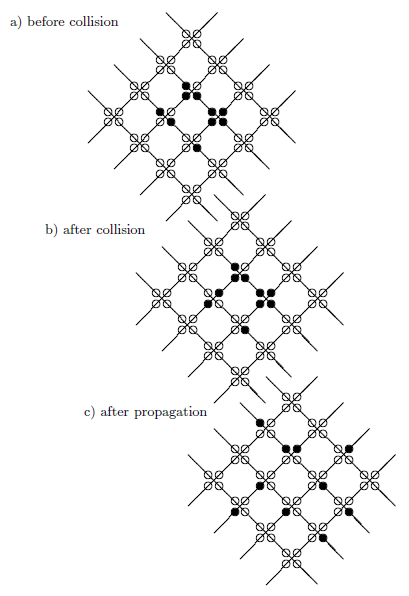
\includegraphics[width=0.60\textwidth]{Screenshots/ImplementationRules-1.PNG}
	\caption{HPP: collision and propagation. Filled circles denote occupied cells and
open circles empty cells. 
a) Part of the lattice before collision (e.g. after propagation);
there is only one collision configuration (two particles in opposite cells at the same node; on the left). 
b) After collision (e.g. before propagation): the configuration of the cells at node on the left side has changed. 
c) After propagation: all particles have moved along the links to their nearest neighbours (the lattice outside the part shown was assumed to be empty, e.g. no propagation of particles from `outside').}
	\label{fig:collision_propagation}
\end{figure}

\begin{figure}[!htp]
	\centering
		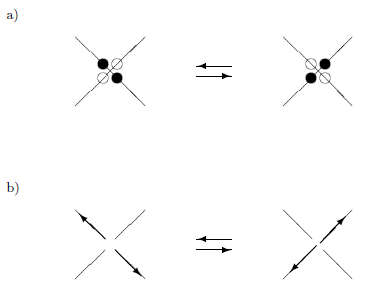
\includegraphics[width=0.60\textwidth]{Screenshots/ImplementationRules-2.PNG}
	\caption{HPP: collisions. 
a) There is only one collision configuration (head-on collision) for HPP: two cell on opposite links are occupied and the two other cells are empty. After collision the formerly empty cells are occupied and vice versa. 
b)Same as a) but showing the associated momentum vectors. Both momentum vectors are rotated by 90°. Mass and momentum are conserved.}
	\label{fig:collisions}
\end{figure}

\section{screenshots, results and comments}

\subsection{Anylogic}

\begin{figure}[!htp]
	\centering
		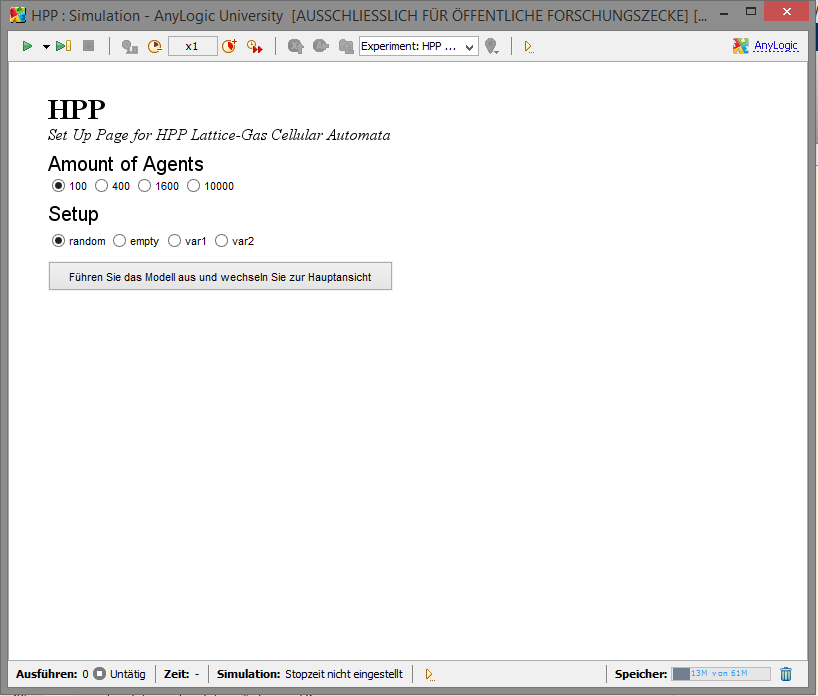
\includegraphics[width=0.60\textwidth]{Screenshots/Anylogic-Start.PNG}
	\caption{Startpage of the Anylogic example. You can choose between different amounts of agents and setups for the HPP Lattice-Gas Simulation.}
	\label{fig:anylogic-start}
\end{figure}

\begin{figure}[!htp]
	\centering
		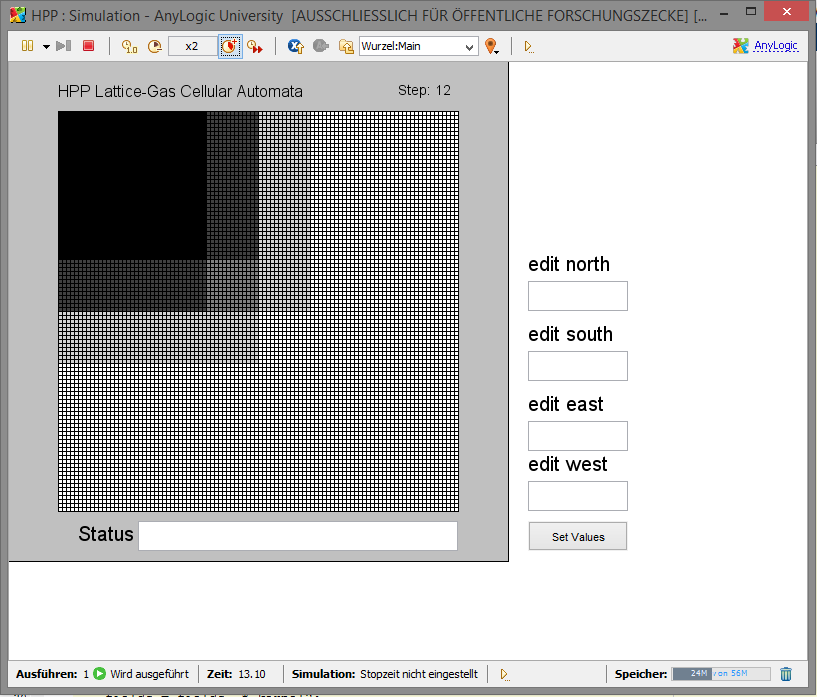
\includegraphics[width=0.60\textwidth]{Screenshots/Anylogic-var1-10000.PNG}
	\caption{Begin of Anylogic Simulation with 10000 Agents and Setup var1. You can edit the values by entering 0 or 1 in the edit field and press set values to see the changes. The status field show if the values are added correctly.}
	\label{fig:anylogic-example1-start}
\end{figure}

\begin{figure}[!htp]
	\centering
		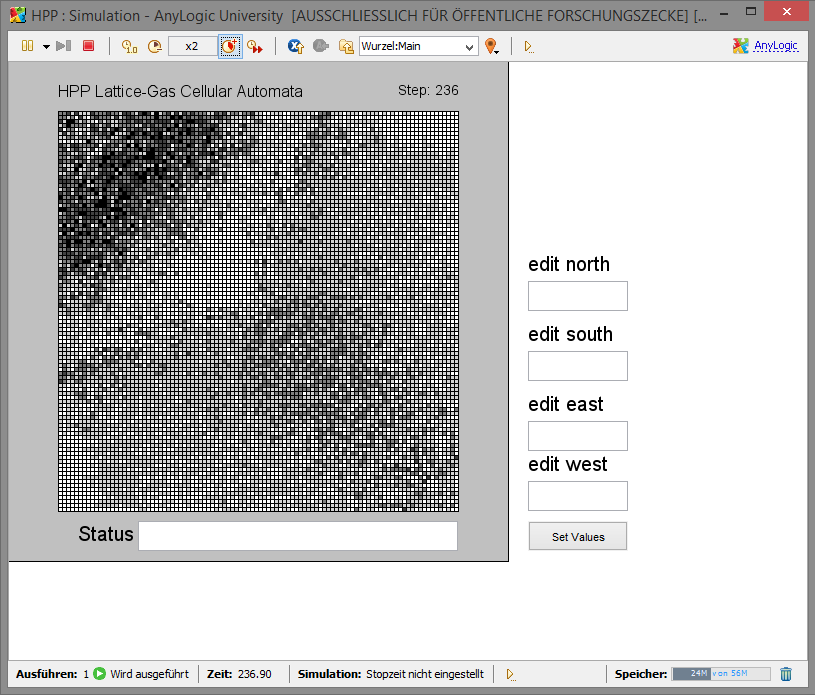
\includegraphics[width=0.60\textwidth]{Screenshots/Anylogic-var1-10000-2.PNG}
	\caption{Anylogic Simulation with 10000 Agents and Setup var1 after 236 steps. Compared with the start image you can see how the gas has distributed.}
	\label{fig:anylogic-example1-end}
\end{figure}

\subsection{MatLab}

\begin{figure}[!htp]
	\centering
		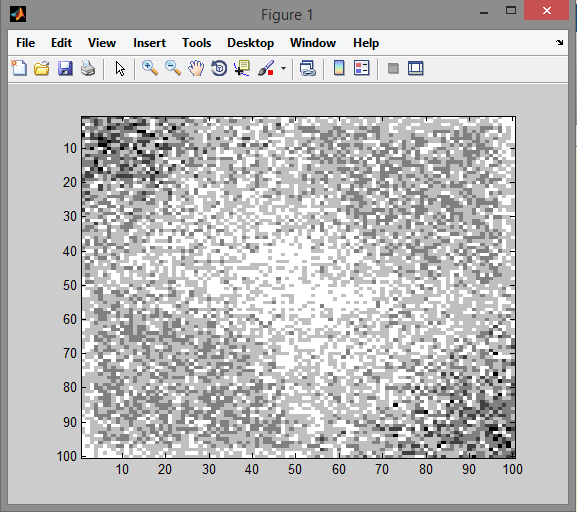
\includegraphics[width=0.60\textwidth]{Screenshots/MatLab-300-100-100-3-Start.PNG}
	\caption{MatLab Simulation with duration of 300 height and width 100 and scenario 3. These 3 values can be changed when the MatLab Simulation is started.}
	\label{fig:matlab-example1-start}
\end{figure}

\begin{figure}[!htp]
	\centering
		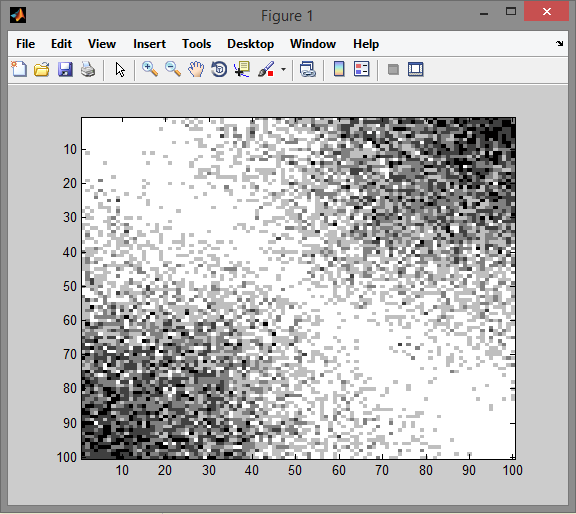
\includegraphics[width=0.60\textwidth]{Screenshots/MatLab-300-100-100-3-End.PNG}
	\caption{MatLab Simulation with duration of 300 height and width 100 and scenario 3. This image shows the state of the HPP LG CA after the duration of 300.}
	\label{fig:matlab-example1-end}
\end{figure}


\end{document}